% ClearVLA — arXiv preprint (ACL style, preprint mode)
\documentclass[11pt]{article}
\usepackage[preprint]{acl}
\usepackage{times}
\usepackage{latexsym}
\usepackage[T1]{fontenc}
\usepackage[utf8]{inputenc}
\usepackage{microtype}
\usepackage{graphicx}
\usepackage{booktabs}
\usepackage{amsmath}
\usepackage{amssymb}
\usepackage{multirow}
\usepackage{array}

\title{Static Pixels Are Not Static Tokens:\\ A Pre-Registered Study of VLA Acceleration on Transparent Lab Objects}

\author{Yogya Mehrotra \\
  \texttt{yogyamehrotra@gmail.com} \\
  \texttt{github.com/yogyam/clearvla}}

\begin{document}
\maketitle

\begin{abstract}
Vision-language-action (VLA) policies are being accelerated with visual-token pruning, cross-observation token caching and low-bit weight quantization, and evaluated almost exclusively on opaque tabletop objects. Laboratory manipulation is dominated by glass, whose thin, low-texture, slowly changing appearance is exactly what these methods discard. We pre-registered the hypothesis that the accelerations cost disproportionately more task success on transparent objects, and built a paired simulated lab testbed to test it: the same seed yields identical scenes with an opaque or a glass test tube (MuJoCo physics, Blender Cycles refraction), three tasks, a fully instrumented 30M-parameter VLA trained on 2,700 scripted demonstrations, and four accelerations implemented on identical weights (FastV-style pruning, VLA-Cache-style pixel-change K/V reuse, INT4 weights, and a ground-truth ``protect'' oracle). Across 3,400 paired closed-loop episodes with the final instrument, offline recall of the object's patches, and latency on an NVIDIA L4 and an Apple M5 Pro, the transparency hypotheses are not supported: at every usable budget no method loses more success on glass than on opaque, quantization is material-neutral within 2 points, and the one significant material effect, at a 12.5\% budget, runs the other way (opaque grasp $-28$ points, glass unchanged). What the study establishes is material-independent. Attention-ranked pruning keeps the object's patches at chance level (24.5\% recall at a 25\% budget) and yet costs almost nothing down to that budget, because the object's information has left the visual tokens by layer 2. Pixel-change caching is catastrophic (0\% grasp and pour at 50\% and 25\% budgets, both materials) because patches whose pixels do not change still have ViT tokens that do (cosine 0.81 to the previous frame); a feature-change criterion fails identically. And none of the three methods reduces wall-clock latency on either device. Data, model, and every episode log are released.
\end{abstract}

\section{Motivation}
\label{sec:motivation}

Efficiency work on VLAs such as OpenVLA and $\pi_0$ \citep{kim2024openvla,black2025pi0} reports success retained under visual-token pruning \citep{liu2025vlapruner,cheng2026vlaiap,yang2025efficientvla}, token caching \citep{xu2025vlacache,wei2026learnedcache} and weight quantization \citep{zhang2026quantvla,wang2026holoq,akbari2026actquant,yan2026hbvla} on LIBERO \citep{liu2023libero}, SIMPLER \citep{li2024simpler} and similar suites, where objects are opaque, textured and well separated from the background \citep{yu2025survey}. Laboratory benchmarks \citep{lan2025autobio,li2025labutopia,ren2026labvla} are full of glassware and name transparent liquids as an open problem, but do not evaluate acceleration. Two adjacent observations made a specific failure plausible. Token-pruning papers note that what gets dropped is ``low-texture edges and narrow contact regions'' \citep{cheng2026vlaiap}; a glass tube is both. And VLA-Cache's own ablation shows that naive reuse of pixel-static tokens costs about ten points of success because task-relevant regions that barely change get cached \citep{xu2025vlacache}; a glass tube changes few pixels as the arm approaches it. If the accelerations discard exactly the evidence a transparent object provides, laboratory deployments would inherit a failure mode that opaque-object benchmarks cannot reveal.

We tested this as a pre-registered study \citep{nosek2018preregistration}: the hypotheses, metrics and decision rules in Table~\ref{tab:hypotheses} were fixed before any model was trained, and the closed-loop design was gated on the cheap offline hypothesis H1. The result is a negative one on the question asked and a positive one on three questions it forced open.

\begin{table}[t]
\centering
\small
\begin{tabular}{>{\raggedright\arraybackslash}p{0.34\columnwidth}>{\raggedright\arraybackslash}p{0.54\columnwidth}}
\toprule
Hypothesis & Supported if \\
\midrule
H1: importance scores under-rank transparent regions & recall of the object's patches at the 25\% budget: opaque $-$ glass $\geq 10$ pts, bootstrap CI excludes 0 \\
H2 (main): speed-ups cost more success on glass & at 25\%, retained success $\geq 15$ pts lower on glass, CI excludes 0, on $\geq 2$ of 3 tasks \\
H3: each method fails where its assumption fails & Cache hurts pour most; Prune hurts grasp most \\
H4: quantization is material-neutral & glass $-$ opaque difference $< 5$ pts \\
H5: protecting instruction-referenced patches recovers the loss & $\geq 50\%$ of the transparency-specific drop recovered at $\leq 10\%$ extra compute \\
\bottomrule
\end{tabular}
\caption{Pre-registered hypotheses. Decision gate: if H1 fails, the closed-loop matrix runs at a single budget with 50 paired episodes per cell instead of the full 5,400-episode design.}
\label{tab:hypotheses}
\end{table}

\paragraph{Contributions.} (1) A paired opaque/glass simulated lab testbed with three tasks and a from-scratch 30M-parameter VLA whose attention maps and key/value caches are fully exposed, so that accelerations can be implemented on identical weights and inspected. (2) Offline and closed-loop evidence, over 3,400 paired episodes with the final instrument (6,300 across all instrument versions), that the transparency hypotheses fail at every usable budget, with a power statement. (3) Three material-independent mechanism findings: pruning keeps the task object at chance yet costs nothing to a 25\% budget; pixel-static patches have non-static ViT tokens, which makes cross-observation K/V reuse catastrophic; and none of the methods moves latency on an L4 or an M5 Pro. (4) A reversed material effect at a 12.5\% budget, reported as an unreplicated observation. (5) The dataset, checkpoint and every episode log, released.

\section{Testbed}
\label{sec:testbed}

\paragraph{Scenes.} Scenes are built per seed with MuJoCo 3.13 \citep{todorov2012mujoco} and the Menagerie Franka Panda \citep{menagerie2022}: a bench, a test tube (radius 14\,mm, height 100\,mm) and one of a rack, a holder or a beaker with an inner fill mark. Per-seed randomisation covers object position ($\pm 5$\,cm), receptacle position ($\pm 3$\,cm), light intensity ($\pm 20\%$) and camera pose ($\pm 1$\,cm, $\pm 2^\circ$). The same seed under \texttt{opaque} and \texttt{glass} gives identical geometry, expert actions and segmentation masks; only the material differs, so every comparison in the paper is paired.

\paragraph{Rendering.} Frames are rendered by Blender 5.2 Cycles \citep{blender2026} driven in-process, with the geometry rebuilt from MuJoCo's tables each episode. Glass uses a Cycles glass BSDF with transparent shadow rays, so the tube appears as faint refraction and a soft shadow rather than a silhouette (Figure~\ref{fig:keepsets}). Two $224^2$ views are used: a fixed diagonal camera and a wrist camera looking down the tool axis. Segmentation masks of the instruction-referenced objects come from MuJoCo's renderer and are pixel-aligned with the Blender frames.

\paragraph{Tasks.} Control runs at 10\,Hz for 300 steps; success must hold for 2\,s. \emph{Grasp-and-rack}: place the tube within 1\,cm of the slot, upright, released. \emph{Pour-to-line}: a scripted liquid model (fill rate proportional to tilt past $55^\circ$; liquid leaves from the lowest point of the mouth's rim; any pour outside the beaker's inner wall is a spill); success is a fill within $\pm 10\%$ of the mark with no spill. \emph{Insert}: the tube starts in the gripper and must be seated in a 30\,mm slot with 1\,mm clearance. Instructions are eight material-neutral paraphrases per task (``put the tube in the rack''). A weld constraint attaches the tube when the gripper closes on it and releases it on open, because the Menagerie finger pads let a tilted tube wedge out during a 10\,s pour; this removes grasp-slip from a perception study and is the device several LeRobot simulation tasks use \citep{cadene2024lerobot}.

\paragraph{Demonstrations.} Scripted waypoint experts (99--100\% success on 100 seeds per cell, both materials) recorded 300 clean episodes per task and material plus 150 recovery episodes per cell in the DART style \citep{laskey2017dart}: 6\,mm execution noise with clean labels. Every fourth control step was rendered in both views: 2,700 episodes and 375k frames.

\paragraph{Instrument.} Model A is a small VLA in the shape of $\pi_0$ and SmolVLA \citep{black2025pi0,shukor2025smolvla}, chosen so that the acceleration hooks are explicit: a frozen SigLIP ViT-B/16 \citep{zhai2023siglip} on each view (392 visual tokens) and a frozen SigLIP text encoder (64 tokens), a 19-D proprioceptive token, a 6-layer $d{=}512$ prefix transformer, and a 4-layer $d{=}384$ flow-matching action expert that cross-attends to the prefix output and predicts a 16-step chunk of 10-D actions (position relative to the current tool centre point, 6-D rotation, gripper). It has 30.4M trainable parameters, was trained for 35k steps (9\,h on an M5 Pro), and runs 10 Euler steps at inference, executing 8 of 16 actions before re-observing. The prefix runs once per observation and exposes every attention map and key/value. Two design changes were required before the model was usable as an instrument, both found by closed-loop tracing: the wrist camera, and actions relative to the current tool position rather than absolute (a 10-pixel tube is smaller than a SigLIP patch; relative targets raised grasp success from 35\% to 80\%). Appendix~\ref{app:versions} lists the versions.

\paragraph{Validity gate.} On 100 unseen paired seeds per cell the instrument reaches grasp 77 / 80\%, insert 98 / 99\% and pour 43 / 37\% (opaque / glass). Pour is below the 60\% bar the design set; its failures are spills at the spout, and the opaque beaker hides its fill level from every viewpoint but straight down, which is the study's only material effect on the base policy. We accepted pour as a weaker instrument rather than spend a fourth training cycle and report it with that caveat.

\paragraph{SmolVLA.} A fine-tuned SmolVLA \citep{shukor2025smolvla} on the same data reached grasp 53 / 48\%, pour 7 / 10\% and insert 52 / 50\%, fitting the demonstrations to 2\,mm offline while approaching 3\,cm off the tube closed-loop. It was not used further; Appendix~\ref{app:smolvla} reports it as a negative result.

\section{Acceleration methods}
\label{sec:methods}

All four methods run inside Model A on identical weights. A budget $b$ is the fraction of the 392 visual tokens (both views, ranked jointly) that receives full prefix compute after layer 2; layers 0--2, the text and proprioceptive tokens, the frozen encoders and the action expert are never touched. This bounds the achievable FLOPs saving at 37\% ($b{=}12.5\%$), which we state rather than hide.

\textbf{Prune} follows FastV \citep{chen2024fastv}: at layer 2, each visual token is scored by the attention it receives from the text and proprioceptive queries, and the top-$b$ are kept for layers 3--6. \textbf{Cache} follows VLA-Cache \citep{xu2025vlacache}: each $16{\times}16$ pixel patch is compared with the same patch in the previous observation (cosine similarity of raw pixels); the $b$ most-changed tokens are recomputed through layers 3--6 while the rest reuse the cached key/value pairs and layer outputs; text and proprioceptive tokens are always recomputed; the first observation of an episode is computed in full. The pixel-change criterion is the assumption under test; a \emph{feature-change} variant ranks tokens by the change of their SigLIP feature vector instead. \textbf{Quant} applies fake INT4 weights, symmetric per group of 64 input channels, to all 84 linear layers of the prefix and expert (8.8\% relative weight error), with fp16 activations. \textbf{Protect} (the H5 oracle) is Prune or Cache with tokens that overlap the simulator's segmentation of the instruction-referenced object ($\geq 25\%$ of the patch) always kept; it is an upper bound by construction.

The 100\% variants of Prune and Cache reproduce the full model bit for bit; a static scene gives zero cache drift; action drift against the full model on demonstration observations is 0.5 / 0.9 / 1.2\,mm median for Prune at 50 / 25 / 12.5\%, 0.8\,mm for INT4, and 4.4\,mm median (p90 22--26\,mm) for Cache. Cost is counted analytically from the token counts each method actually uses, and latency is measured (\S\ref{sec:latency}).

\section{Results}
\label{sec:results}

\subsection{Importance scores under-rank everything, not glass}
\label{sec:h1}

\begin{figure*}[t]
\centering
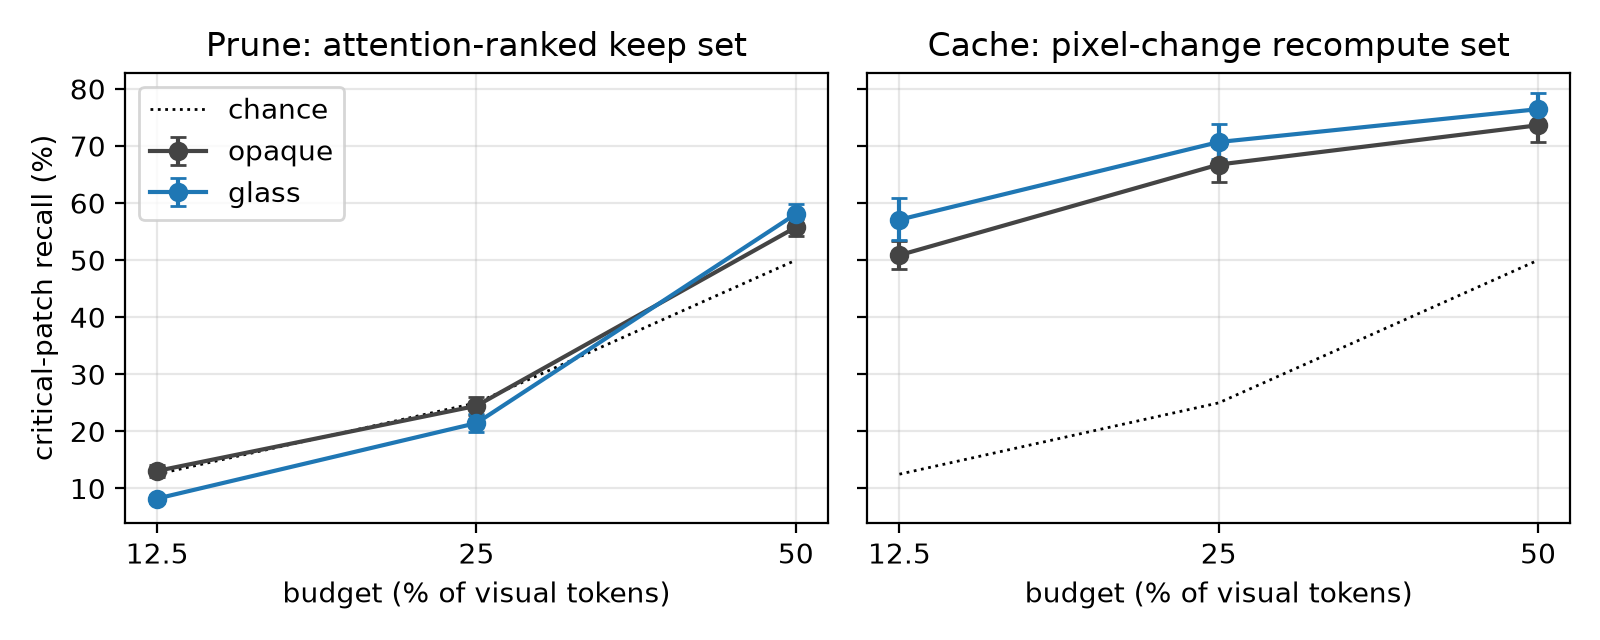
\includegraphics[width=0.85\textwidth]{figures/fig3_h1_recall.png}
\caption{Critical-patch recall of the keep set vs.\ budget (50 unseen paired seeds per task, 2,623 observations per material, 95\% bootstrap CIs over episodes). Prune (left) sits on the chance line for both materials; Cache (right) is above chance and higher for glass.}
\label{fig:h1}
\end{figure*}

\begin{figure}[t]
\centering
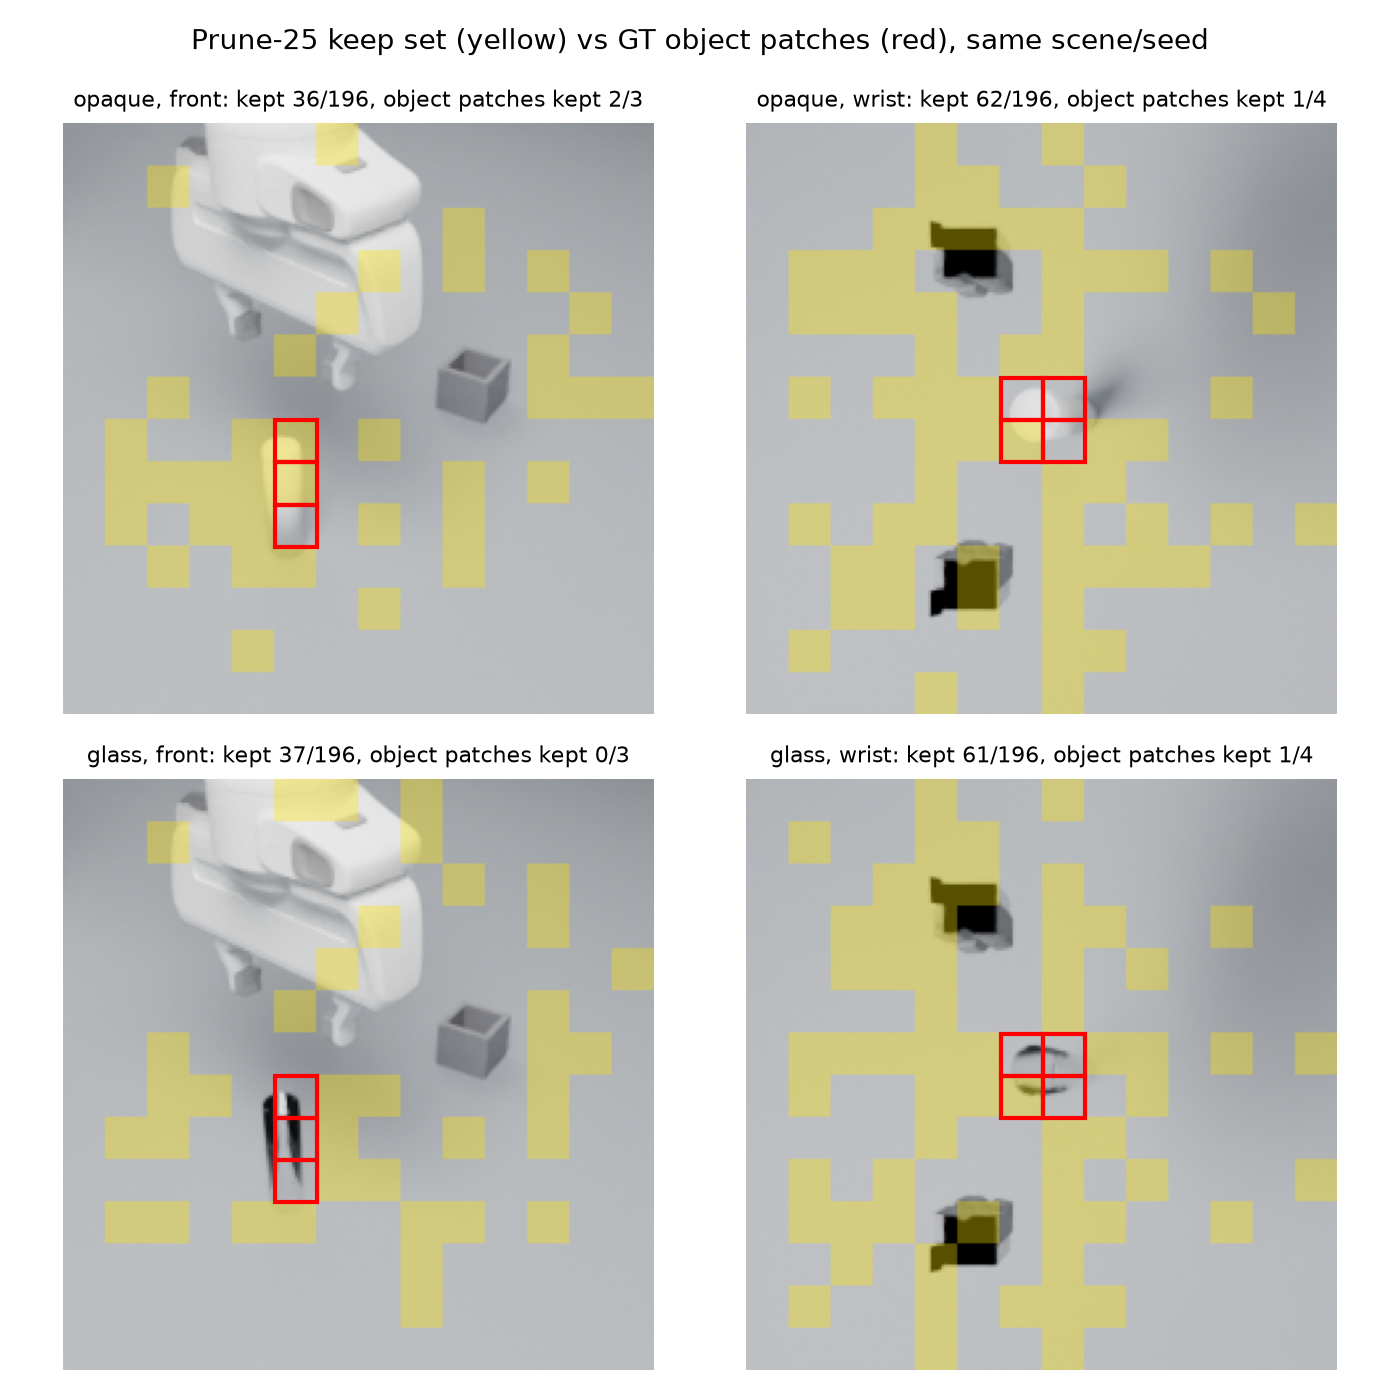
\includegraphics[width=\columnwidth]{figures/fig1_keep_sets.png}
\caption{The same scene and seed under both materials, both views; Prune-25 keep set in yellow, ground-truth object patches outlined in red. The opaque front view keeps 2 of 3 object patches, the glass front view 0 of 3; the wrist view keeps 1 of 4 in both.}
\label{fig:keepsets}
\end{figure}

The offline set is the scripted expert driving the 50 unseen seeds 1000--1049 of every task under both materials, with both views rendered at every observation point a policy would see: 2,623 observations per material, identical frames for every method and identical trajectories across materials because the expert is state-driven. A patch is \emph{critical} if at least 25\% of its pixels lie on the instruction-referenced object; recall is the fraction of critical patches in the keep set (Figure~\ref{fig:h1}, Table~\ref{tab:h1}).

\begin{table}[t]
\centering
\small
\setlength{\tabcolsep}{4pt}
\begin{tabular}{lccc}
\toprule
At 25\% budget & Opaque & Glass & Gap [95\% CI] \\
\midrule
Prune & 24.5 & 21.5 & $+3.0$ [$+1.8$, $+4.2$] \\
Cache & 66.8 & 70.7 & $-3.9$ [$-4.5$, $-3.4$] \\
\bottomrule
\end{tabular}
\caption{Critical-patch recall (\%) at the pre-registered 25\% budget, pooled over tasks and views; gap $=$ opaque $-$ glass with a paired bootstrap over seeds (10k resamples).}
\label{tab:h1}
\end{table}

H1 is not supported: the gap is $+3.0$ points against a bar of 10. The more informative number is the level. Prune keeps 24.5\% of the object's patches at a 25\% budget, which is chance; only 0.6--4.7\% of layer-2 attention from the text and proprioceptive queries lands on the object at all. The glass tube receives about half the attention mass of the opaque one (2.1\% vs.\ 4.7\% on grasp), which is the effect the hypothesis predicted, but it is small and concentrated in grasp ($+8.0$ points at 25\%, $+9.7$ at 12.5\%). Cache goes the other way: the glass tube refracts the moving arm and background, so its patches change \emph{more} pixels between observations and are recomputed more often (on pour at 12.5\%: 70\% opaque vs.\ 88\% glass). The premise that glass changes pixels less than it changes state is not what the renders show.

\subsection{Speed-ups cost the same on glass}
\label{sec:matrix}

\begin{table*}[t]
\centering
\small
\begin{tabular}{lcccccc}
\toprule
& \multicolumn{2}{c}{Grasp} & \multicolumn{2}{c}{Pour} & \multicolumn{2}{c}{Insert} \\
\cmidrule(lr){2-3}\cmidrule(lr){4-5}\cmidrule(lr){6-7}
Configuration & Opaque & Glass & Opaque & Glass & Opaque & Glass \\
\midrule
Full & 84 & 82 & 42 & 28 & 92 & 100 \\
Prune-50 & 84 & 78 & 28 & 20 & 98 & 100 \\
Prune-25 & 76 & 78 & 34 & 32 & 94 & 100 \\
Prune-12.5 & \textbf{56} & \textbf{82} & 40 & 50 & 92 & 96 \\
Protect-prune-25 (oracle) & 80 & 76 & 46 & 26 & 90 & 96 \\
Cache-50 (pixel) & 0 & 2 & 0 & 0 & 48 & 66 \\
Cache-25 (pixel) & 0 & 0 & 0 & 0 & 22 & 24 \\
Cache-25 (feature) & 0 & 0 & 0 & 0 & 12 & 20 \\
Quant INT4 & 76 & 74 & 38 & 22 & 94 & 100 \\
\bottomrule
\end{tabular}
\caption{Closed-loop success (\%) on 50 paired unseen seeds per cell (seeds 1000--1049; synchronous evaluation; horizon 300). Per-cell 95\% CIs span about $\pm 14$ points; full tables with CIs are in Appendix~\ref{app:tables}.}
\label{tab:matrix}
\end{table*}

\begin{figure*}[t]
\centering
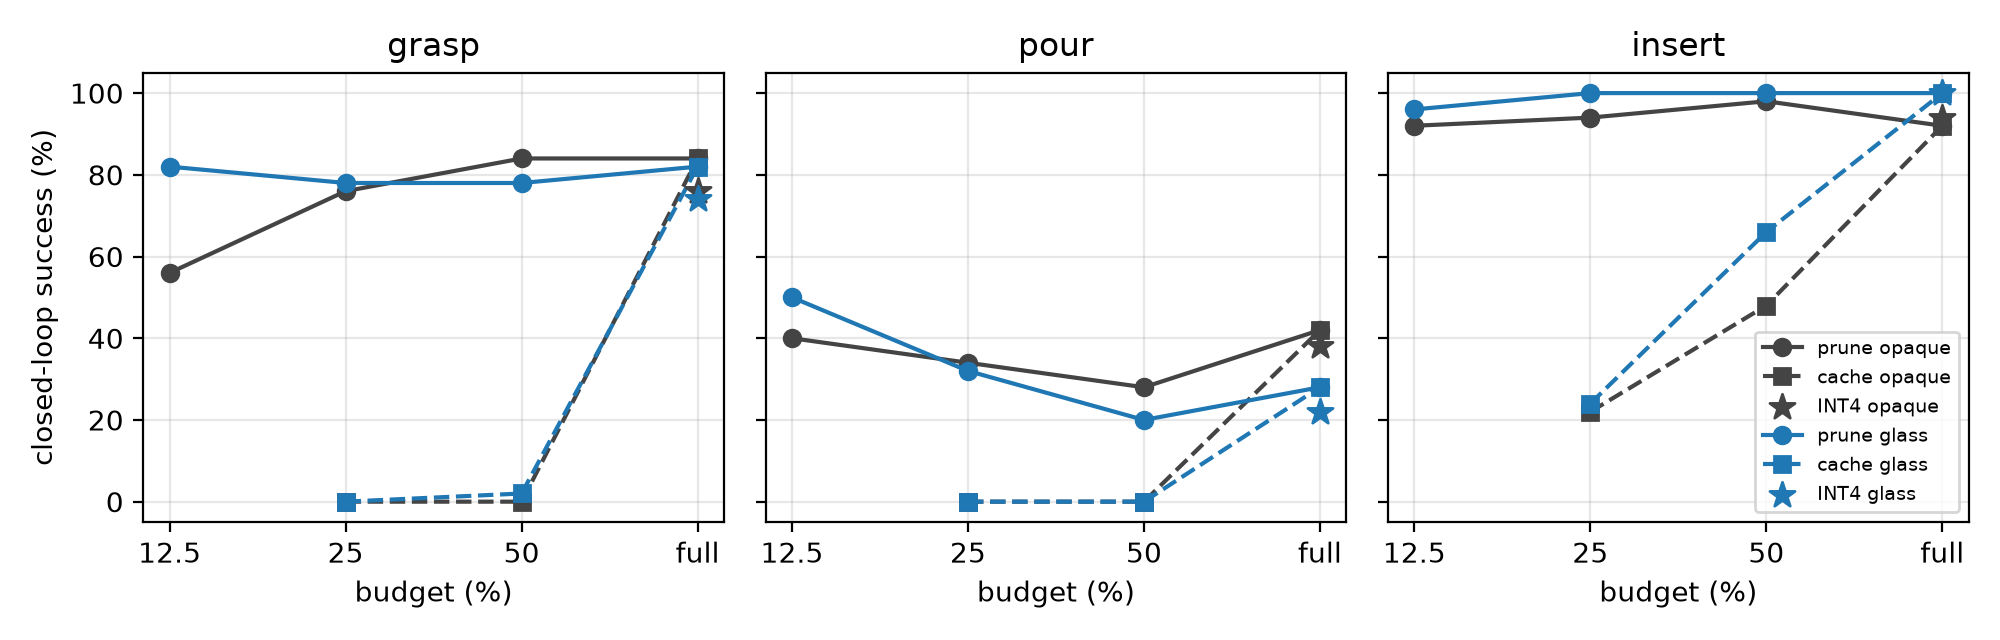
\includegraphics[width=\textwidth]{figures/fig2_budget_curve.png}
\caption{Closed-loop success vs.\ budget per task; circles Prune, squares Cache, stars INT4; black opaque, blue glass. Prune is flat to 25\% on every task and both materials; Cache is at the floor at 50\% and 25\%; INT4 tracks Full.}
\label{fig:budget}
\end{figure*}

\begin{table}[t]
\centering
\small
\begin{tabular}{llr@{\ }l}
\toprule
Config & Task & DiD & [95\% CI] \\
\midrule
Prune-25 & grasp & $-4$ & [$-26$, $+18$] \\
 & pour & $-12$ & [$-34$, $+8$] \\
 & insert & $+2$ & [$-6$, $+10$] \\
Prune-12.5 & grasp & $\mathbf{-28}$ & [$-52$, $-4$] \\
 & pour & $-24$ & [$-48$, $0$] \\
 & insert & $+4$ & [$-6$, $+16$] \\
Cache-25 & pour & $-14$ & [$-32$, $+4$] \\
Quant INT4 & grasp & $0$ & [$-18$, $+18$] \\
 & pour & $+2$ & [$-26$, $+28$] \\
 & insert & $+2$ & [$-8$, $+12$] \\
\bottomrule
\end{tabular}
\caption{Material difference-in-differences: (success $-$ Full) on opaque minus the same on glass, in points, paired over seeds with a 10k bootstrap. A negative value means glass lost \emph{less}. Rows not shown lie within $\pm 6$ with CIs spanning zero.}
\label{tab:did}
\end{table}

The pre-registered matrix (Full, Prune-25, Cache-25, Quant, plus the feature-change cache and the Protect oracle) ran on 50 paired seeds per cell, 1,800 episodes; three further budgets added 900 (Table~\ref{tab:matrix}, Figure~\ref{fig:budget}). The paired material difference-in-differences are in Table~\ref{tab:did}.

\textbf{H2 is not supported.} At the 25\% budget no method loses more on glass than on opaque; every CI includes zero. With $n{=}50$ per cell the study excludes glass-specific losses of roughly 20 points or more, not smaller ones. \textbf{H3} has the pre-registered direction for Prune, whose largest loss is on grasp ($-8$ / $-4$ points), but the loss is small; Cache floors every task on both materials, so its task ordering is uninformative. \textbf{H4 is supported}: INT4 costs the same on both materials within 2 points. (The pre-registered ratio metric, retained success, gives $+12$ on pour with a CI of $[-75, +90]$, an artefact of dividing by a 28\% base rate; absolute differences are reported alongside it in Appendix~\ref{app:tables}.) \textbf{H5 is not applicable}: there is no transparency-specific loss to recover, and the oracle that keeps 100\% of the object's patches at the same budget lands within noise of plain Prune-25 on every cell, which is itself informative (\S\ref{sec:implications}).

\subsection{A reversal at 12.5\%}
\label{sec:reversal}

The one significant material effect in the study appears at the most aggressive budget and runs opposite to H2: opaque grasp falls by 28 points while glass does not move (DiD $-28$ $[-52, -4]$), and glass pour rises. This is one budget, $n{=}50$, and one of 18 comparisons, so we report it as an observation. It is consistent with the H1 numbers: at 12.5\% the keep set retains 13\% of the opaque tube's patches and 8\% of the glass tube's, yet only the opaque policy suffers, so success on glass at this budget cannot depend on the tube's own patches. A plausible reading is that the glass tube's evidence, its shadow, its refraction and the background it distorts, is spread over more of the image than an opaque silhouette and survives chance-like pruning better; we did not test this.

\subsection{Static pixels are not static tokens}
\label{sec:cache}

\begin{figure*}[t]
\centering
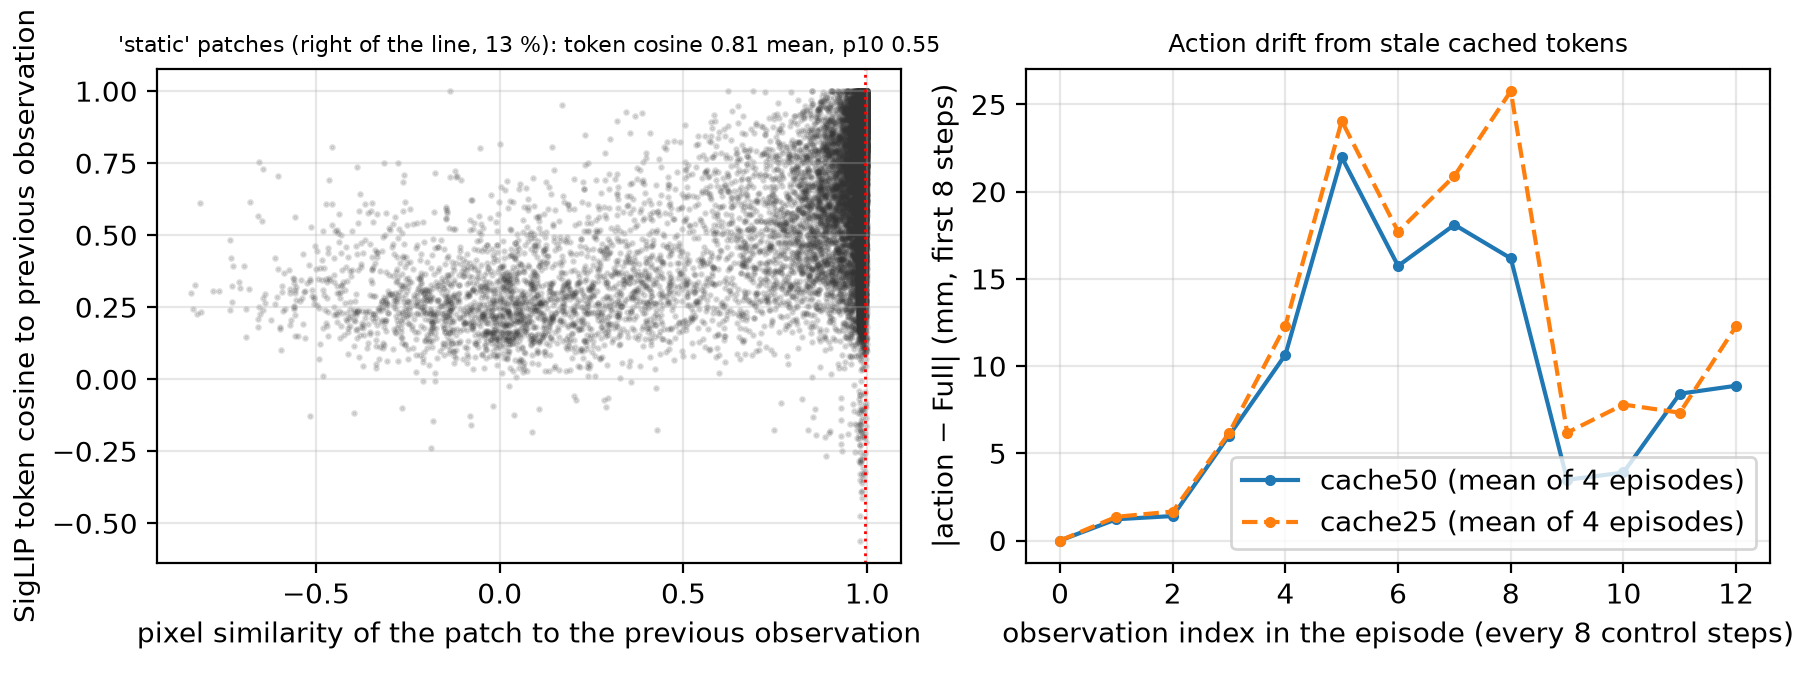
\includegraphics[width=\textwidth]{figures/fig4_cache_staleness.png}
\caption{Left: pixel similarity of a patch to the previous observation vs.\ the cosine of its SigLIP token to the previous observation, over consecutive expert observations; 13\% of patches are pixel-static (right of the dotted line) and their tokens still move (cosine 0.81 mean, tenth percentile 0.55). Right: action drift of Cache-50 and Cache-25 against the full model along expert episodes, mean of four grasp episodes.}
\label{fig:cache}
\end{figure*}

Cache scores 0\% on grasp and pour at both 50\% and 25\% budgets, on both materials, and nine of ten failures knock the tube over. Figure~\ref{fig:cache} shows why. A ViT token depends on the whole image, not on its own pixels: among patches whose pixels are static between consecutive observations (similarity above 0.995, 13\% of patches), the SigLIP token's cosine to its previous value is 0.81 on average and below 0.55 for a tenth of them. Reusing key/value pairs for pixel-static tokens therefore feeds the prefix stale features on every frame in which anything moved, which in manipulation is every frame. The drift accumulates along the approach (1 to 23\,mm over the first six observations at a 50\% budget), the arm arrives 2--3\,cm off, and the tube is knocked over. The feature-change variant fails identically (Table~\ref{tab:matrix}), so it is the reuse, not the pixel criterion, that breaks the policy. VLA-Cache's published version filters reuse by attention and reports about ten points of loss from naive reuse on its benchmark \citep{xu2025vlacache}; for a policy that depends on a 10-pixel object, naive reuse is not a ten-point loss but a total one. Transparency never enters.

\subsection{Nothing is faster}
\label{sec:latency}

\begin{table*}[t]
\centering
\small
\begin{tabular}{lrrrrr}
\toprule
NVIDIA L4, budget & Tokens & GFLOPs & Eager & CUDA graphs & TensorRT \\
\midrule
Full & 457 & 24.4 & 64.8 & 5.44 & 5.51 \\
Prune-50 & 261 & 19.0 & 65.3 & 5.17 & 5.72 \\
Prune-25 & 163 & 16.5 & 64.1 & 4.88 & 5.82 \\
Prune-12.5 & 114 & 15.3 & 64.1 & 4.67 & 6.05 \\
SigLIP, two views & -- & $\approx 67$ & 7.3 & 2.5 & -- \\
\bottomrule
\end{tabular}\\[6pt]
\begin{tabular}{lrrrr}
\toprule
Apple M5 Pro, config & SigLIP & Prefix & Expert & Total \\
\midrule
Full & 27.8 & 4.5 & 18.9 & 51.4 \\
Prune-25 & 28.6 & 5.8 & 20.2 & 54.6 \\
Prune-12.5 & 28.6 & 5.8 & 20.6 & 55.0 \\
Cache-25 & 28.7 & 5.6 & 20.8 & 54.9 \\
Quant INT4 (fake) & 28.8 & 4.8 & 20.7 & 54.2 \\
\bottomrule
\end{tabular}
\caption{Latency per observation in ms (batch 1, median of 300 runs). Top: NVIDIA L4, prefix $+$ 10 expert steps; tokens $=$ tokens after layer 2; GFLOPs analytic for prefix $+$ expert; eager fp16 autocast, \texttt{torch.compile} with CUDA graphs, and TensorRT fp16. Bottom: Apple M5 Pro, eager PyTorch on MPS, by stage (SigLIP on two views; expert $=$ 10 Euler steps).}
\label{tab:latency}
\end{table*}

Table~\ref{tab:latency} measures the accelerated region (prefix and 10-step expert) at batch~1. Eager execution on the L4 is launch-bound: 65\,ms whatever the token count. Removing launch overhead with CUDA graphs or TensorRT is a $12\times$ speed-up by itself; after that, a 37\% FLOPs reduction from pruning buys 14\% of latency under CUDA graphs and nothing under TensorRT, whose per-layer fixed costs dominate at these sizes. On the M5 Pro the frozen vision encoder is 55\% of the observation time and the ten-step expert 37\%; the prefix the methods touch is 9\%, and pruning or caching add gather overhead rather than save time. Fake INT4 changes nothing by construction; a real INT4 kernel would save weight bandwidth, which is not the bottleneck for a 30M-parameter model at batch~1. For a policy of this size, none of the three methods is a latency lever, on either device.

\section{Related Work}
\label{sec:related}

\paragraph{Token pruning for VLAs.} FastV \citep{chen2024fastv} showed that a vision-language model can drop half its visual tokens after layer 2 with little loss, and VLA variants \citep{liu2025vlapruner,cheng2026vlaiap,yang2025efficientvla} report success retained on LIBERO and SIMPLER at 25--50\% of tokens. VLA-IAP \citep{cheng2026vlaiap} measures retention of gripper--object boundary tokens, the closest mechanistic argument to H1, but never varies material. Our finding that the object's patches are kept at chance yet success survives (\S\ref{sec:h1}, \S\ref{sec:matrix}) suggests that boundary-token retention is not what makes pruning work in a small trained-from-scratch policy.

\paragraph{Token caching.} VLA-Cache \citep{xu2025vlacache} reuses key/value pairs of pixel-static tokens with an attention-based relevance filter, and its ablation of naive reuse is the closest published point to \S\ref{sec:cache}; a learned successor \citep{wei2026learnedcache} decides which tokens to cache. Neither reports the token-level drift of pixel-static patches under a ViT encoder that we measure.

\paragraph{Quantization and compression fragility.} Post-training quantization of VLAs to W4A4 and below \citep{zhang2026quantvla,wang2026holoq,akbari2026actquant,yan2026hbvla} reports closed-loop error compounding at low bit widths; our H4 result agrees that 4-bit weights are benign for a small model and adds that the cost is material-neutral. \citet{jabbour2025scissors} find the vision backbone far more fragile than the language model under weight pruning; our observation that the object's information leaves the visual tokens by layer 2 is a token-side counterpart.

\paragraph{Lab benchmarks and transparency.} AutoBio \citep{lan2025autobio}, LabUtopia \citep{li2025labutopia} and LabVLA \citep{ren2026labvla} build laboratory simulators and benchmarks with glassware and name transparent liquids as a gap, without acceleration; SEVO \citep{fang2026sevo} grasps transparent bottles with active illumination and no opaque control. Robustness suites \citep{morgan2026colosseum,fei2025liberoplus} vary colour, texture, lighting and distractors but not transparency and not accelerated models. To our knowledge no prior work evaluates an acceleration method as a function of object transparency; this study does, and finds the effect absent at the budgets where the methods are usable.

\section{Limitations}
\label{sec:limitations}

\begin{itemize}
\item \textbf{Simulated glass is easier than real glass.} Cycles renders clean refraction with no sensor noise, no specular highlights from laboratory lighting and no depth-sensor failure. A real-glass replication could reveal effects the simulator cannot.
\item \textbf{The liquid is scripted, not simulated,} and the pour instrument is below the 60\% validity bar (43 / 37\%). Pour results carry wider effective uncertainty than their CIs suggest.
\item \textbf{Power.} $n{=}50$ per cell bounds the detectable glass-specific loss at about 20 points. Smaller effects, including the $+3$-point H1 gap and the $+8$-point grasp gap, are real but below the pre-registered bar.
\item \textbf{One model, one seed, one data regime.} The reversed effect at 12.5\% is unreplicated and is one of 18 comparisons.
\item \textbf{Bounded saving by design.} Layers 0--2, the encoders and the expert are untouched, so the achievable FLOPs reduction is 37\%; a method that prunes before the encoder would face the object-localisation problem this design side-steps.
\item \textbf{Oracle masks and synchronous evaluation.} Protect and the H1 masks use simulator segmentation; the simulator pauses during inference, so latency cannot affect success.
\item \textbf{The sticky-gripper weld} removes grasp-slip as a failure mode, as in several LeRobot simulation tasks.
\item \textbf{SmolVLA was not diagnosed to the root.} The negative result in Appendix~\ref{app:smolvla} identifies the closed-loop failure but not which of the frozen VLM, the 64-token image budget or the per-frame action convention causes it.
\end{itemize}

\section{Implications}
\label{sec:implications}

For someone about to accelerate a laboratory VLA, the study replaces one worry with two. Material is not the variable to test first: at every budget where pruning and quantization keep the policy usable, glass and opaque objects lose the same. The variables to test are the interaction between the vision encoder and any cross-observation cache, and the latency budget itself. On the first, a frozen ViT makes every token a function of the whole image, so ``static'' is a property of tokens, not of pixels, and a cache must be validated by token drift, not pixel change; the feature-change variant shows that even a token-level criterion does not rescue reuse when three quarters of the tokens stay stale. On the second, a 30M-parameter policy at batch~1 spends its time in the encoder, the iterative expert and kernel launches, none of which token methods touch; the honest speed-up in Table~\ref{tab:latency} came from compilation, not from any of the three methods.

Two methodological points follow. Recall of the task object's patches, the quantity H1 was built on and the one that pruning papers often argue from, did not predict closed-loop success here: the object's information had already left the visual tokens by the layer at which pruning acts, and an oracle that kept every object patch changed nothing. And pre-registration is what makes the negative result usable: the hypotheses, the bar and the decision gate were fixed in advance, the gate was triggered, and the three mechanism findings were not what the study was looking for.

\section*{Reproducibility}

{\raggedright\emergencystretch=2em
All code, the pre-registered plan (\texttt{PLAN.md}), the weekly logs, every closed-loop episode (6,300 JSONL records across all instrument versions, 3,400 with the final one, with per-observation keep sets, object-patch recall and FLOPs) and the analysis scripts are at \url{https://github.com/yogyam/clearvla}; \texttt{scripts/reproduce.md} maps every table and figure to one command, and the analysis-only path runs in minutes without a simulator. The dataset (LeRobot v3, 2,700 episodes, both views, CC BY 4.0) is at \url{https://huggingface.co/datasets/yogyamehrotra/clearvla-sim} and the Model A v4 checkpoint at \url{https://huggingface.co/yogyamehrotra/clearvla-model-a-v4}. Total compute: about 60\,h of M5 Pro time and \$9 of cloud GPU.
\par}

\bibliography{refs}
\bibliographystyle{acl_natbib}

\appendix

\section{SmolVLA as a second instrument}
\label{app:smolvla}

\texttt{lerobot/smolvla\_base} \citep{shukor2025smolvla,cadene2024lerobot} was fine-tuned on the same 2,700 episodes, with our cameras mapped to its \texttt{camera1}/\texttt{camera2} slots, $224^2$ frames padded to $512^2$, and actions as per-frame deltas because the LeRobot format stores one action per frame; 20k steps at batch 64 on an H100 (101\,min), with only the 100M-parameter action expert trainable (the library default). On 100 unseen paired seeds per cell it reached grasp 53 / 48\%, pour 7 / 10\% and insert 52 / 50\% (opaque / glass), against 77 / 80, 43 / 37 and 98 / 99 for Model A v4. Offline it reproduces the demonstrations to 2.0 / 1.9 / 2.6\,mm per axis with correct gripper timing; closed-loop it descends 3\,cm to the side of the tube without correcting laterally. Re-observing every 4 or 2 steps instead of 8 did not help (7 / 20 vs.\ 6 / 20 grasp on the same seeds). We attribute the gap to the frozen web-pretrained VLM (64 visual tokens per $512^2$ image) and the per-frame action convention, and did not spend further budget on it.

\section{Instrument versions}
\label{app:versions}

v1: front camera only, absolute-pose actions, 150 demonstrations per cell; grasp 39 / 33\%, pour 8 / 7\%. v2: added the wrist camera and 150 demonstrations per cell; no closed-loop improvement despite 3--6\,mm offline error, and a trace showed the gripper closing 23--31\,mm off the tube. v3: actions relative to the current tool position; grasp 80 / 82\%, insert 98 / 96\%, pour 10 / 22\%. v4: 150 DART recovery demonstrations per cell; grasp 77 / 80\%, pour 43 / 37\%, insert 98 / 99\% (the instrument used throughout). The offline error of v2 (3--6\,mm) and its closed-loop failure are the same signature later seen in SmolVLA.

\section{Full tables}
\label{app:tables}

Per-cell 95\% bootstrap CIs, the pre-registered ratio-based diff-in-difference, failure-mode histograms, per-view and per-task H1 recall, and the budget-curve tables are in the repository: \texttt{results/week5/matrix\_report.md}, \texttt{results/week6/matrix\_report.md}, \texttt{results/week4/h1\_report.md}. Representative CIs: Full grasp 84 [74, 94] / 82 [70, 92]; Full pour 42 [28, 56] / 28 [16, 40]; Cache-25 grasp 0 [0, 0] / 0 [0, 0]; Prune-12.5 grasp 56 [42, 70] / 82 [70, 92].

\end{document}
